\documentclass{beamer}
\usepackage[utf8]{inputenc}
\usepackage{ragged2e}
\usepackage{graphicx}
\usepackage{caption}
\usepackage{placeins}
\usepackage{todonotes}
\usepackage{subcaption}
\usepackage[font=footnotesize,labelformat=simple]{subcaption}

\usetheme{Madrid}
\usecolortheme{default}

%------------------------------------------------------------
%This block of code defines the information to appear in the
%Title page
\title[Slide deck - Colombia] %optional
{Slide deck - Colombia}

\subtitle{Proposed outline}



\institute{World Bank} % (optional)


\date[WB 2024] % (optional)
{Conference, December 2024}


%End of title page configuration block
%------------------------------------------------------------



%------------------------------------------------------------
%The next block of commands puts the table of contents at the 
%beginning of each section and highlights the current section:

\AtBeginSection[]
{
  \begin{frame}
    \frametitle{Table of Contents}
    \tableofcontents[currentsection]
  \end{frame}
}
%------------------------------------------------------------


\begin{document}

%The next statement creates the title page.
\frame{\titlepage}


%---------------------------------------------------------
%This block of code is for the table of contents after
%the title page
\begin{frame}
\frametitle{Table of Contents}
\tableofcontents
\end{frame}
%---------------------------------------------------------
\section{Regional heterogeneity}

%---------------------------------------------------------
%---------------------------------------------------------

\begin{frame}
\frametitle{Regional heterogeneity}
\begin{figure}[!htb]
\justifying
  \caption{Alternative informality definitions}
  \centering
  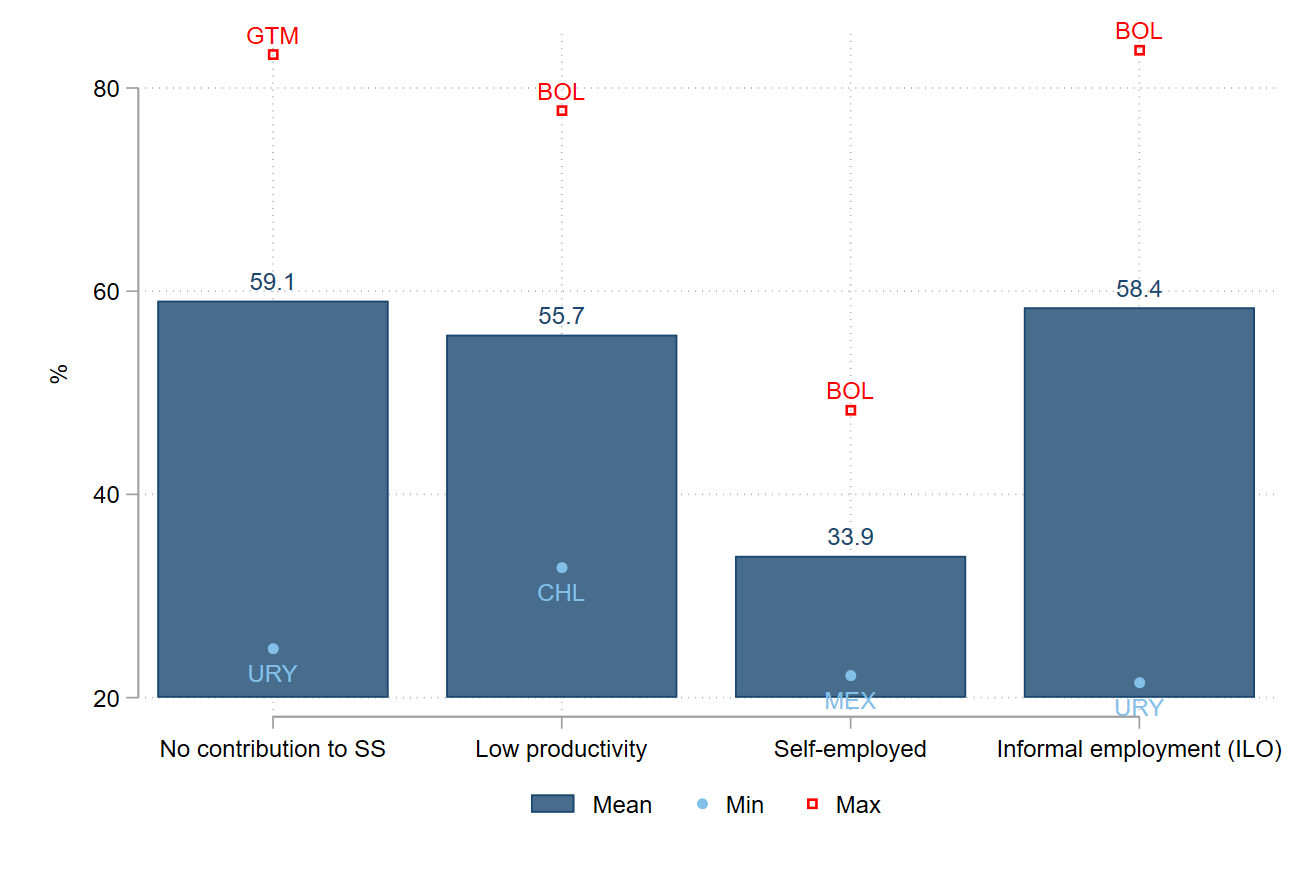
\includegraphics[width=0.8\linewidth]{latex/figures/Snapshot/Alternative informality definitions_CASEN.png}
  \label{fig:informaldefs}
\end{figure}
  \centering
\footnotesize{Source: Household Surveys-SEDLAC and ILO.}


\end{frame}
%--------------------------------------------------------
%---------------------------------------------------------

\begin{frame}
\frametitle{Regional heterogeneity}
\begin{figure}[!htb]
\justifying
  \caption{Informality (legal definition) and GDP per capita}
  \centering
  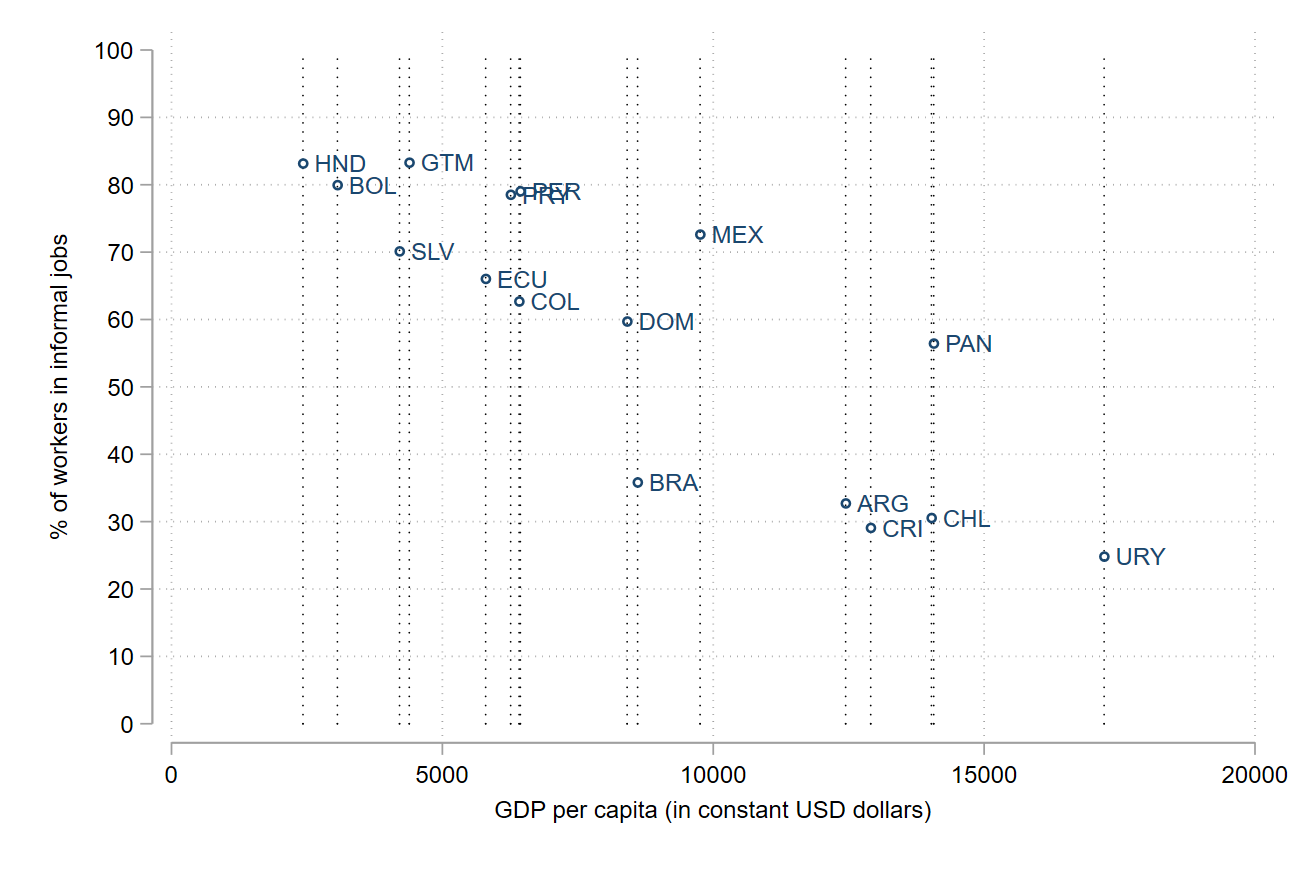
\includegraphics[width=0.8\linewidth]{latex/figures/Snapshot/GDP vs informal_ss.png}
  \label{fig:GDPinformalSS}
\end{figure}
  \centering
\footnotesize{Source: Household Surveys-SEDLAC and World Bank.}


\end{frame}
%--------------------------------------------------------
%---------------------------------------------------------

\begin{frame}
\frametitle{Regional heterogeneity}
\begin{figure}[!htb]
\justifying
  \caption{Informality (productive definition) and GDP per capita}
  \centering
  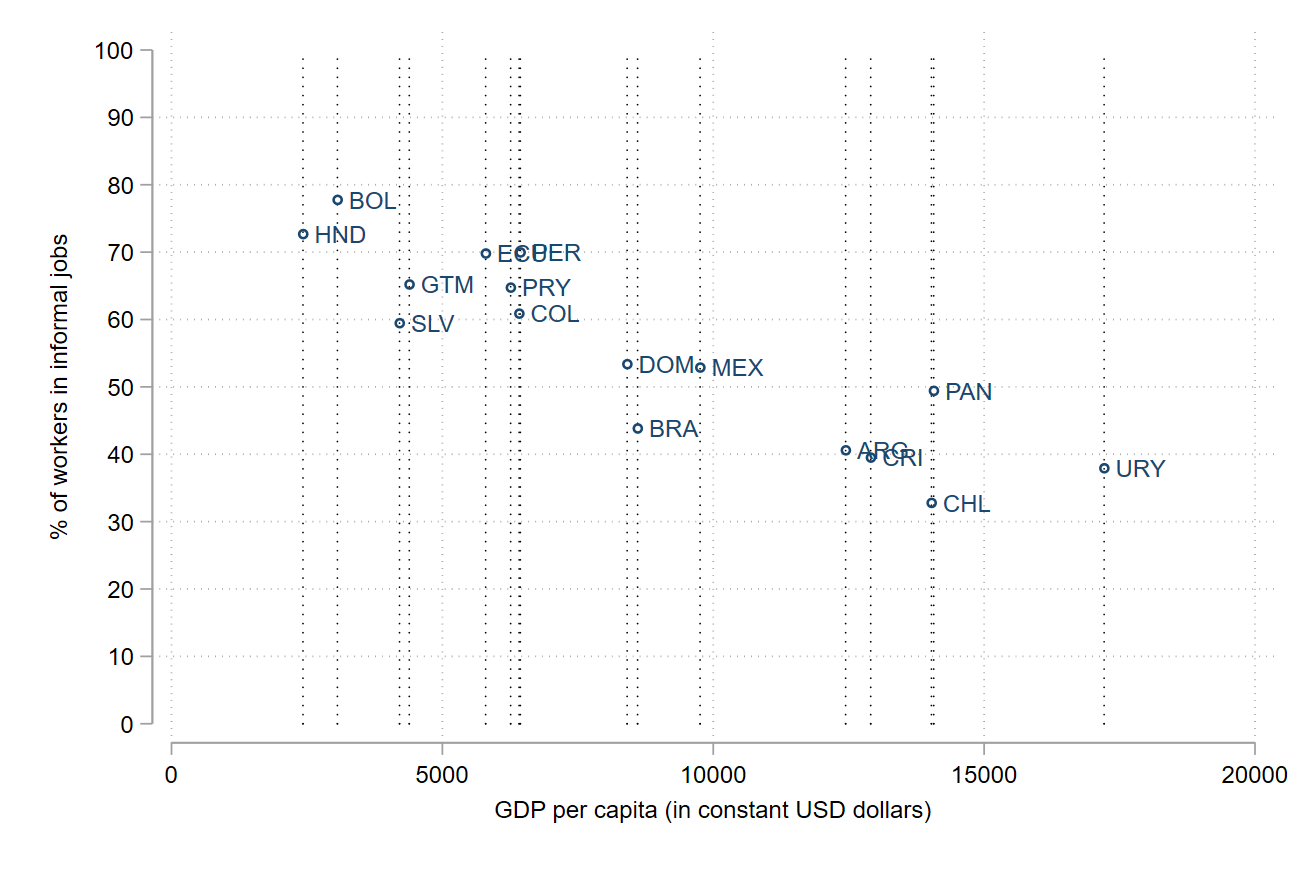
\includegraphics[width=0.8\linewidth]{latex/figures/Snapshot/GDP vs informal_pr.png}
  \label{fig:GDPinformalpr}
\end{figure}
  \centering
\footnotesize{Source: Household Surveys-SEDLAC and World Bank.}


\end{frame}
%--------------------------------------------------------

%--------------------------------------------------------

\begin{frame}
\frametitle{Regional heterogeneity}
\begin{figure}[!htb]
\justifying
  \caption{Structure of labor market}
  \centering
  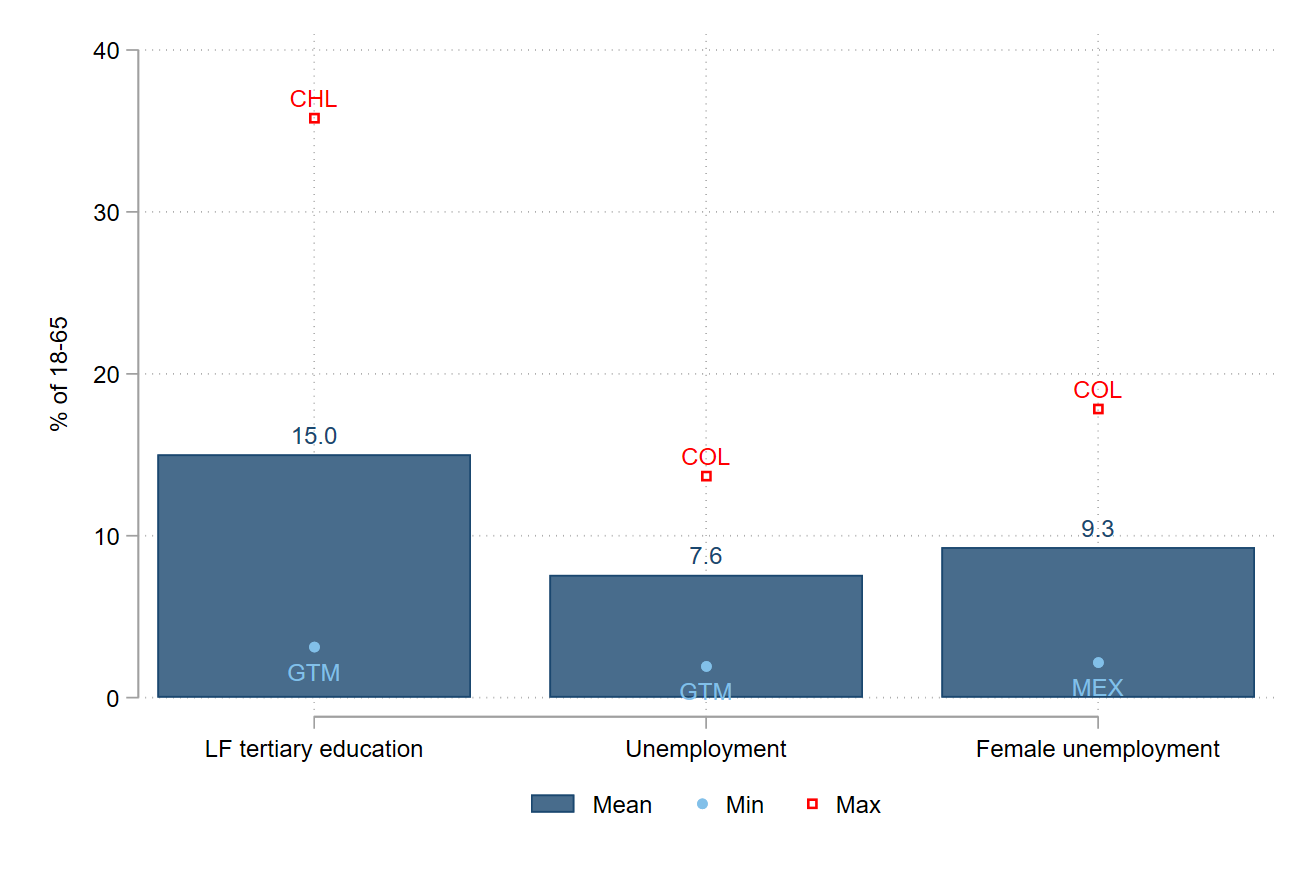
\includegraphics[width=0.8\linewidth]{latex/figures/Snapshot/Structure of labor market_b.png}
  \label{fig:labmarket2}
\end{figure}
  \centering
\footnotesize{Source: Household Surveys-SEDLAC.}


\end{frame}
%---------------------------------------------------------

%---------------------------------------------------------
\begin{frame}
\frametitle{Regional heterogeneity}
 \begin{figure}[!htb]
        \justifying
        \caption{Structure of employment}     
        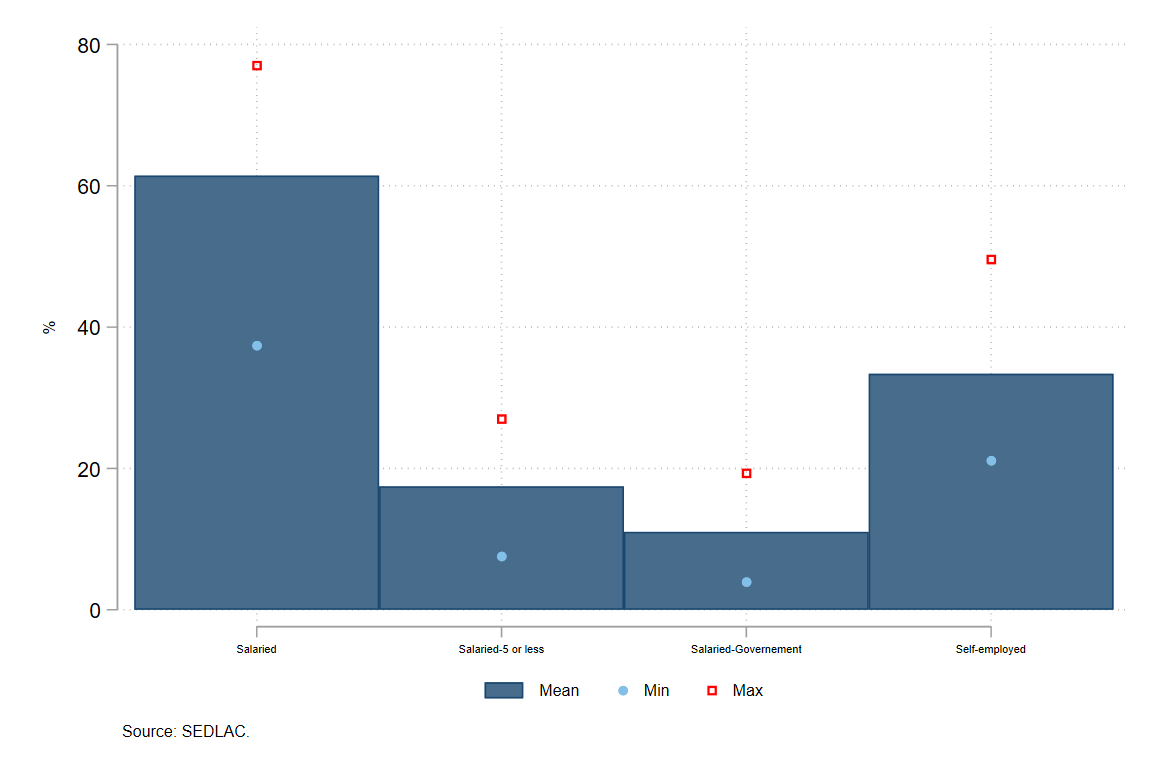
\includegraphics[width=0.8\linewidth]
        {latex/figures/Snapshot/Structure of employment.png}
        \label{fig:employment}
        \centering
        \footnotesize{Source: Household Surveys-SEDLAC.}
\end{figure}
\end{frame}
%---------------------------------------------------------
     
%---------------------------------------------------------
\begin{frame}
\frametitle{Regional heterogeneity}
\begin{figure}[!htb]
        \justifying
        \caption{Structure of employment by sector}     
        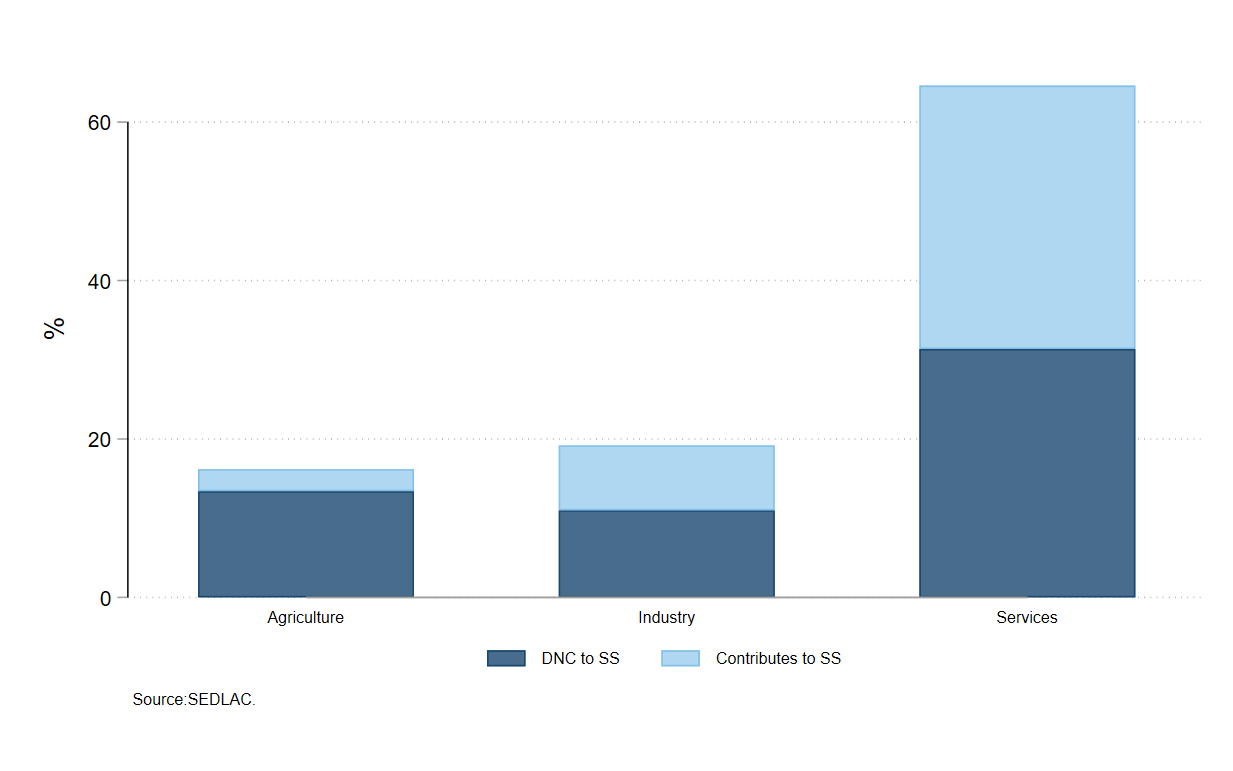
\includegraphics[width=0.8\linewidth]{latex/figures/Snapshot/Structure of employment and sector.png}
        \label{fig:sector}
        \centering
       \footnotesize{Source: Household Surveys-SEDLAC.}

\end{figure}
\end{frame}
%---------------------------------------------------------

%---------------------------------------------------------
\begin{frame}
\frametitle{Regional heterogeneity}
\begin{figure}[!htb]
        \justifying
        \caption{Structure of private employment by firm size}     
        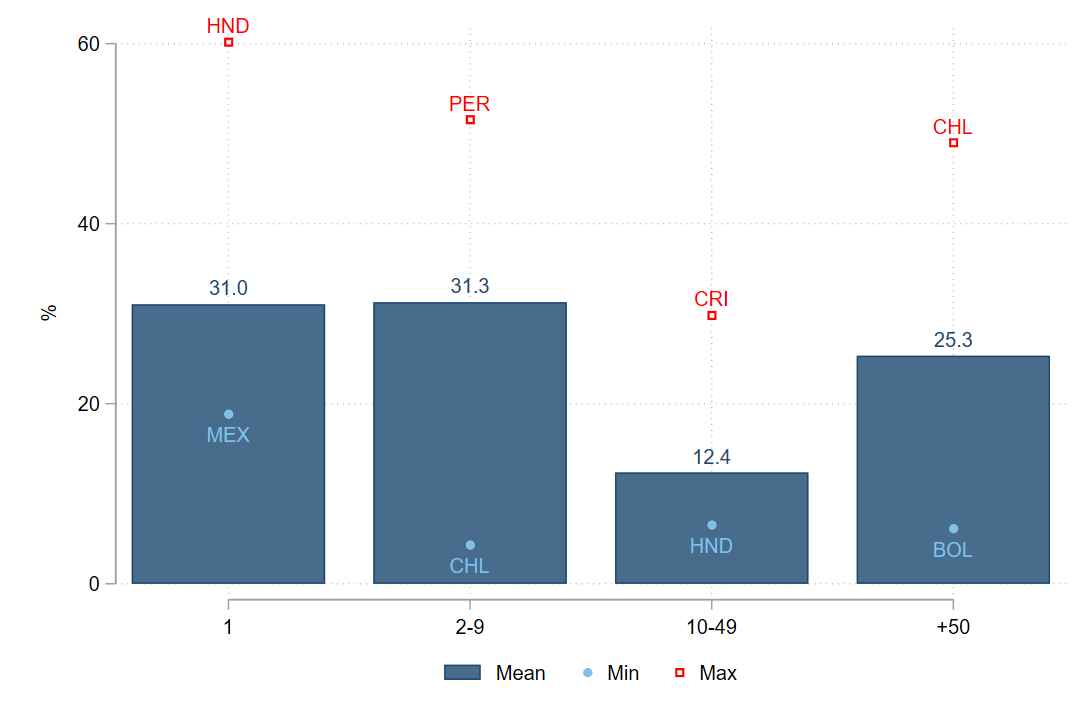
\includegraphics[width=0.8\linewidth]{latex/figures/Snapshot/Structure of employment by firm size.png}
        \label{fig:firmsize}
        \centering
        \footnotesize{Source: Household Surveys-SEDLAC.}
        \end{figure}

\end{frame}
%---------------------------------------------------------
%---------------------------------------------------------
\begin{frame}
\frametitle{Regional heterogeneity}
\begin{figure}[!htb]
        \justifying
        \caption{Share of Workers Who Do Not Contribute to Social Security by Selected Characteristics}     
        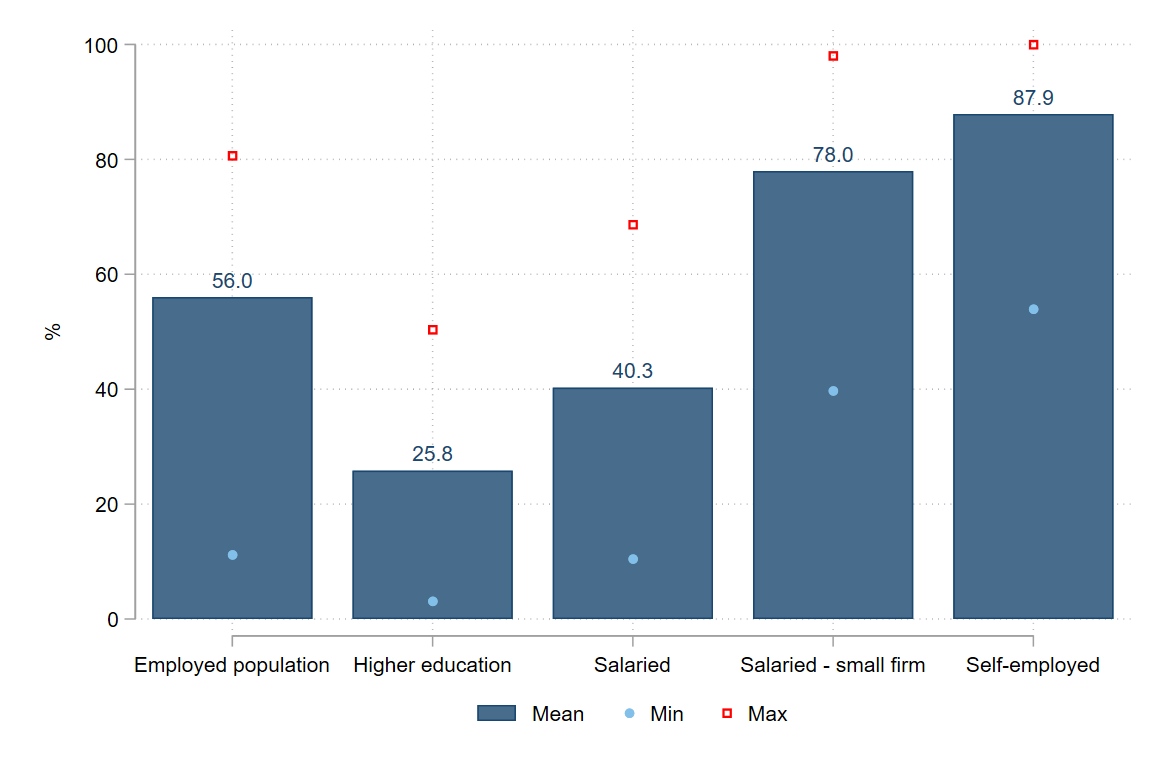
\includegraphics[width=0.8\linewidth]{latex/figures/Snapshot/Social security contributions.png}
        \label{fig:SScontributions}
        \centering
        \footnotesize{Source: Household Surveys-SEDLAC.}
 \end{figure}
 \end{frame}
%---------------------------------------------------------
%---------------------------------------------------------


\section{2021 vs 2005}

%---------------------------------------------------------

\begin{frame}
\frametitle{Changes over time}
\begin{figure}[!htb]
    \justifying
     \caption{Workers who do not contribute to SS}     
     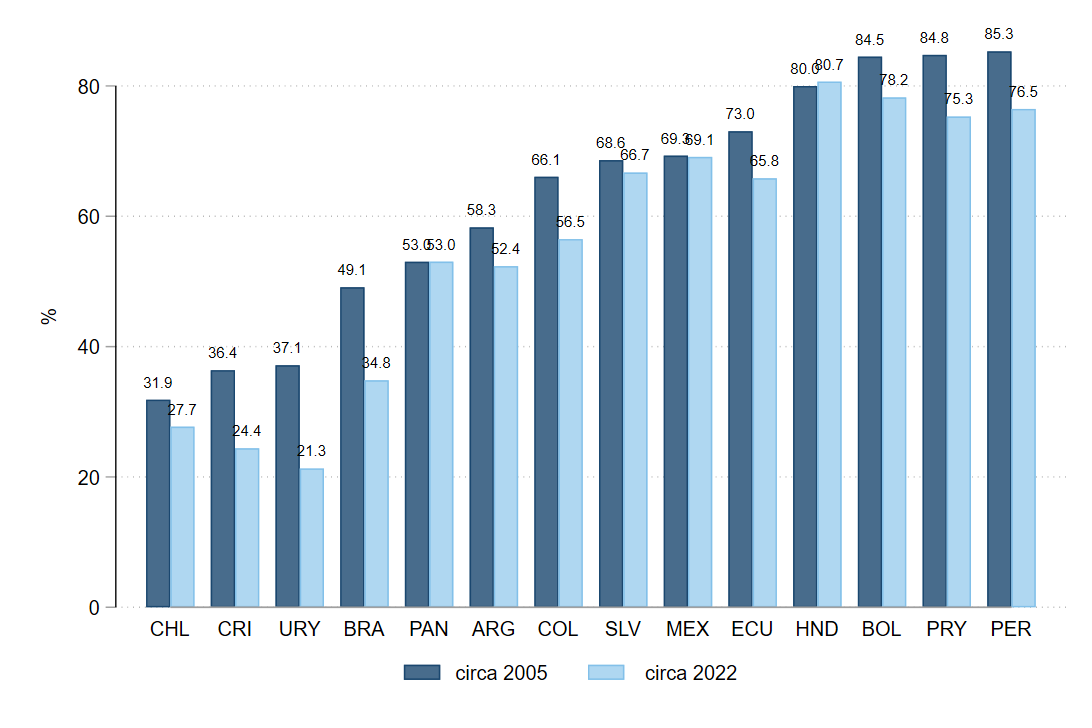
\includegraphics[width=0.8\linewidth]{latex/figures/Snapshot/snapshot_informal_ss.png}
    \label{fig:SalariedSS}
    \centering
    \footnotesize{Source: Household Surveys-SEDLAC.}
\end{figure}
    
\end{frame}

%---------------------------------------------------------
%---------------------------------------------------------

\begin{frame}
\frametitle{Changes over time}
\begin{figure}[!htb]
    \justifying
     \caption{Workers who work at small firms}     
     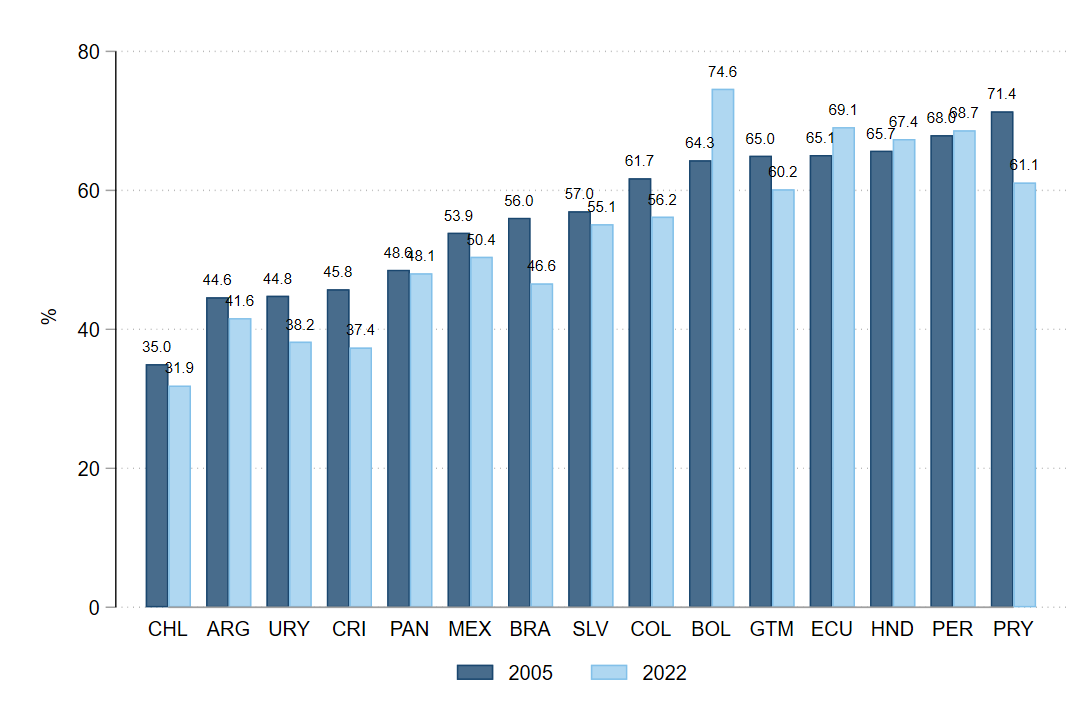
\includegraphics[width=0.8\linewidth]{latex/figures/Snapshot/snapshot_workers_small.png}
    \label{fig:SalariedSmall}
    \centering
    \footnotesize{Source: Household Surveys-SEDLAC.}
\end{figure}
\end{frame}
%---------------------------------------------------------
%---------------------------------------------------------

\begin{frame}
\frametitle{Changes over time}
\begin{figure}[!htb]
    \justifying
     \caption{Salaried who do not contribute to SS}     
       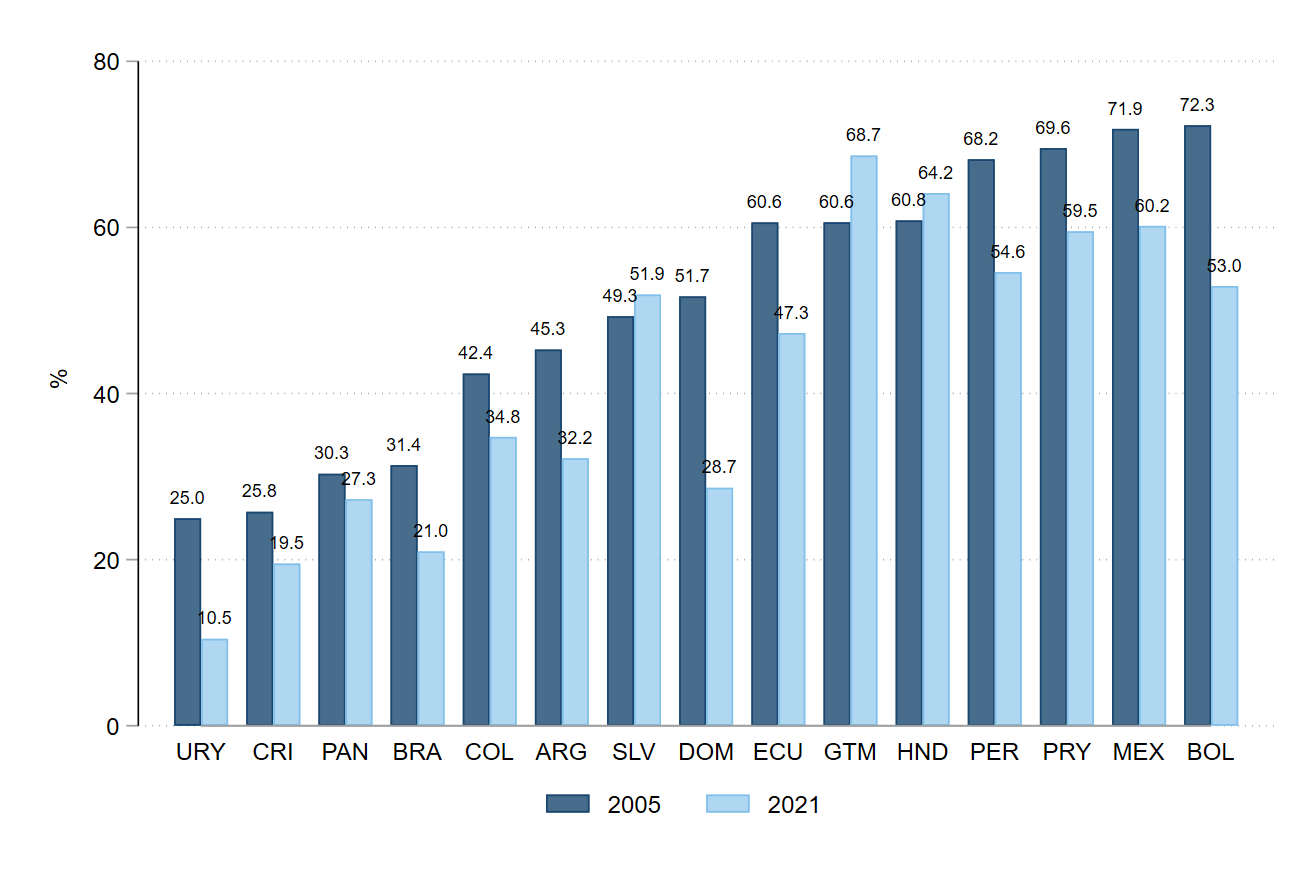
\includegraphics[width=0.8\linewidth]
       {latex/figures/Snapshot/snapshot_informal_ss_dep.png}
    \label{fig:SalariedSS}
    \centering
    \footnotesize{Source: Household Surveys-SEDLAC.}
\end{figure}


    
\end{frame}

%---------------------------------------------------------
%---------------------------------------------------------

\begin{frame}
\frametitle{Changes over time}
\begin{figure}[!htb]
    \justifying
     \caption{Salaried who work at small firms}     
     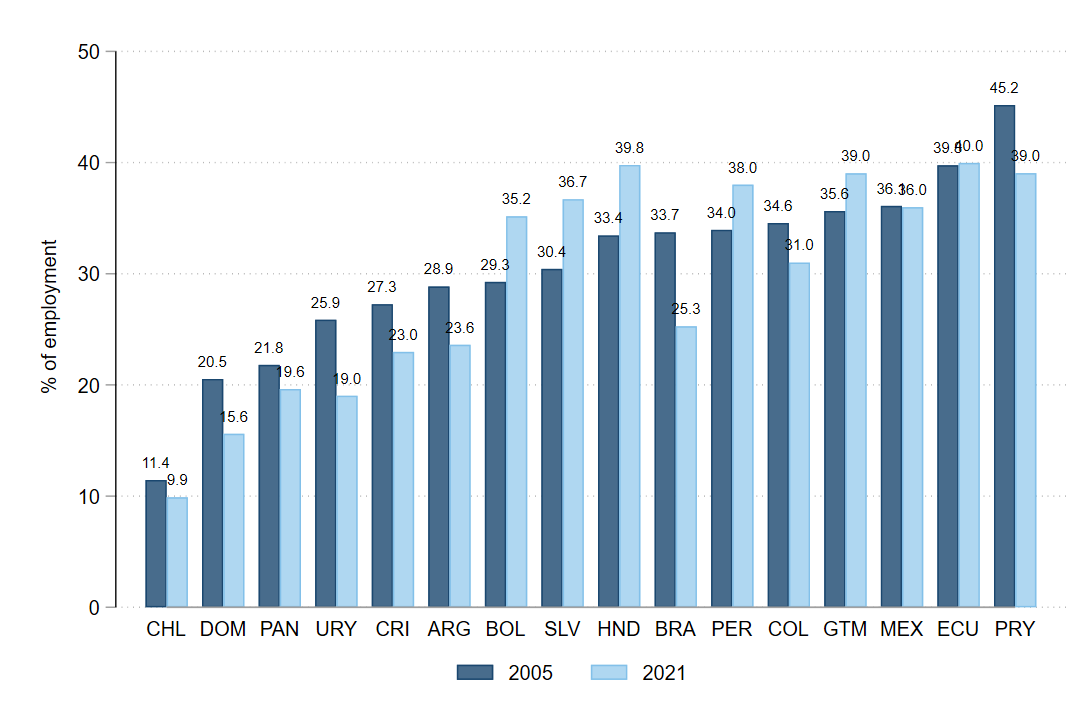
\includegraphics[width=0.8\linewidth]{latex/figures/Snapshot/snapshot_dependents_small.png}
    \label{fig:SalariedSmall}
    \centering
    \footnotesize{Source: Household Surveys-SEDLAC.}
\end{figure}
\end{frame}
%---------------------------------------------------------

%---------------------------------------------------------

\section{Dynamics: last 20 years}  
%---------------------------------------------------------
%---------------------------------------------------------
\begin{frame}
\frametitle{Dynamics: last 20 years}
\begin{figure}[!htb]
        \justifying
        \caption{Evolution of alternative informality related measures}     
        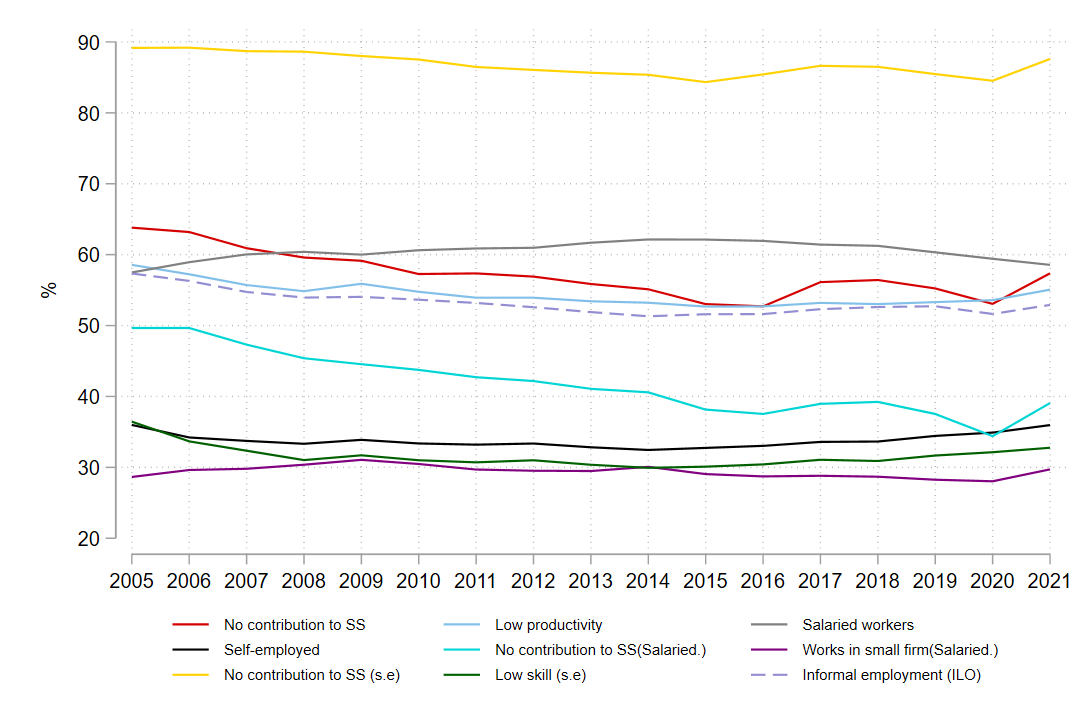
\includegraphics[width=0.8\linewidth]{latex/figures/Evolution/informality_evolution_LAC.png}
        \label{fig:EvolutionLAC}
        \centering
        \footnotesize{Source: Household Surveys-SEDLAC and ILO.}
 \end{figure}
 \end{frame}
%---------------------------------------------------------
%---------------------------------------------------------
\begin{frame}
\frametitle{Time series: last 20 years}
\begin{figure}[!htb]
        \justifying
        \caption{Workers who do not contribute to SS by country}     
        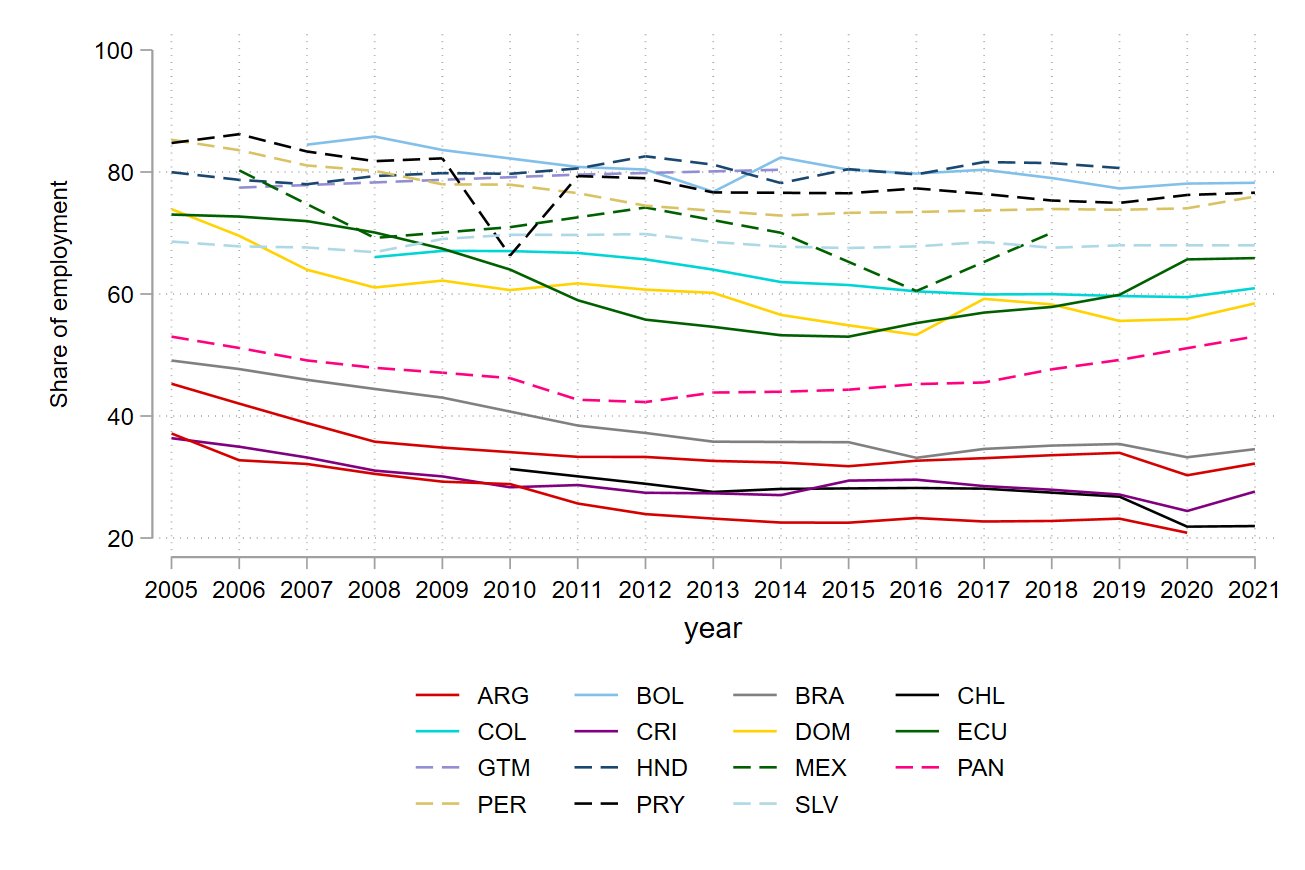
\includegraphics[width=0.8\linewidth]{latex/figures/Evolution/informal_ss_all.png}
        \label{fig:Evolution_informalSS}
        \centering
        \footnotesize{Source: Household Surveys-SEDLAC.}
 \end{figure}
 \end{frame}
%---------------------------------------------------------
%---------------------------------------------------------
\begin{frame}
\frametitle{Dynamics: last 20 years}
\begin{figure}[!htb]
        \justifying
        \caption{Workers who are low skill self-employed or are employed at a small firm or zero wage workers by country}     
        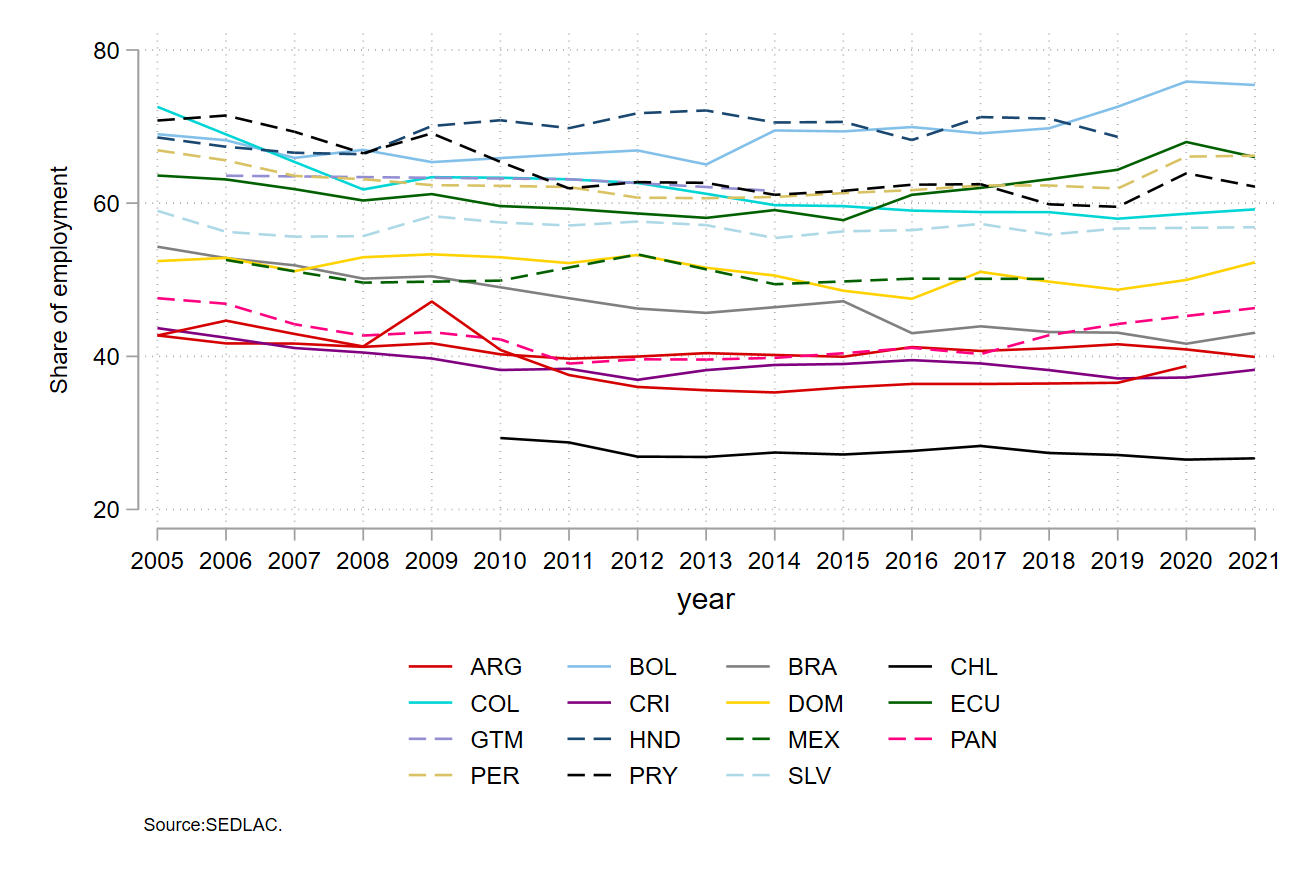
\includegraphics[width=0.8\linewidth]{latex/figures/Evolution/informal_pr_all.png}
        \label{fig:Evolution_informalpr}
        \centering
        \footnotesize{Source: Household Surveys-SEDLAC.}
 \end{figure}
 \end{frame}
%---------------------------------------------------------
%---------------------------------------------------------
\begin{frame}
\frametitle{Dynamics: last 20 years}
\begin{figure}[!htb]
        \justifying
        \caption{Salaried workers who do not contribute to SS by country}     
        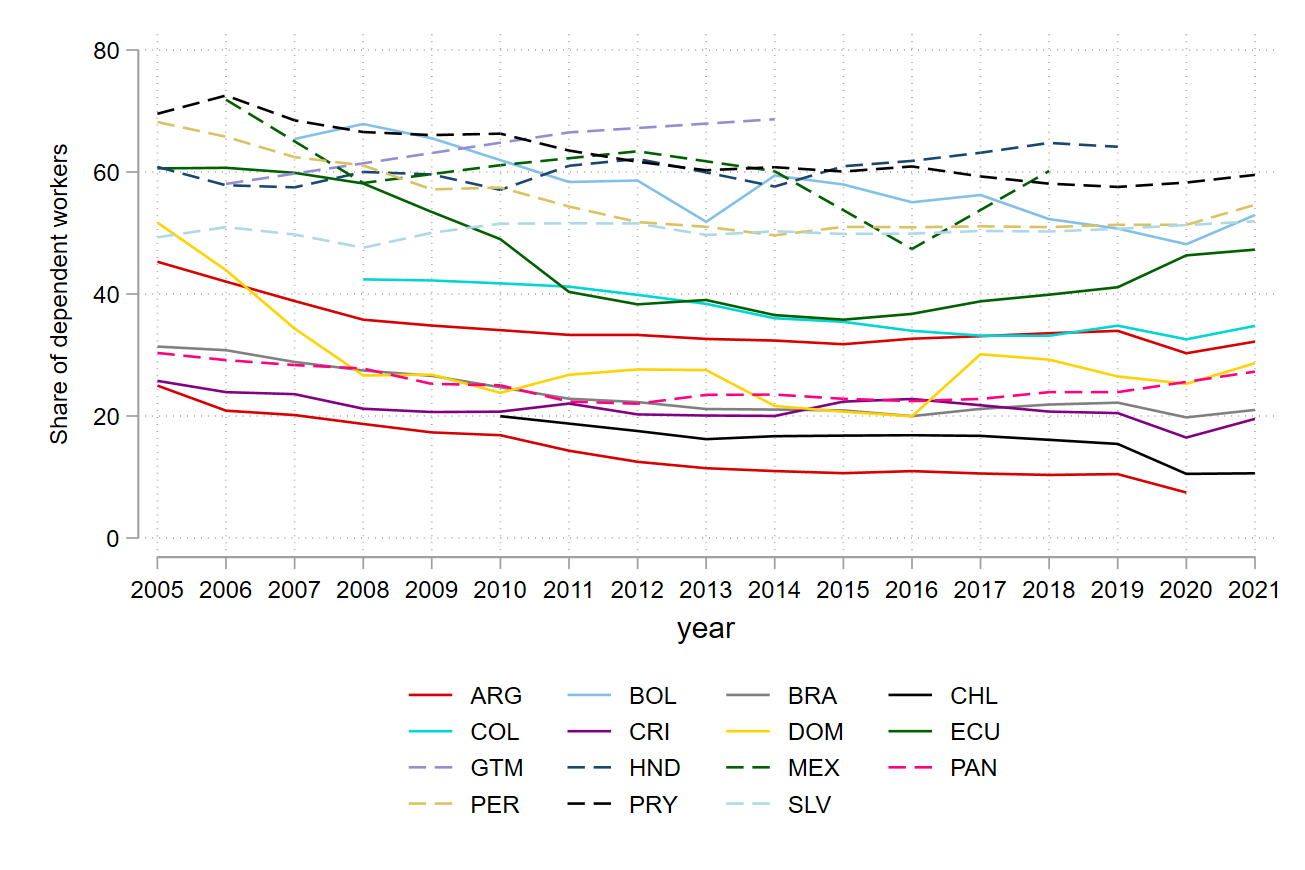
\includegraphics[width=0.8\linewidth]{latex/figures/Evolution/informal_ss_dep_all.png}
        \label{fig:Evolution_informalssdep}
        \centering
        \footnotesize{Source: Household Surveys-SEDLAC.}
 \end{figure}
 \end{frame}
%--------------------------------------------------------
%-----------------------------------------------------------------------------------------------------------------
%--------------------------------------------------------
%---------------------------------------------------------
%---------------------------------------------------------
\begin{frame}
\frametitle{Dynamics: last 20 years}
\begin{figure}[!htb]
        \justifying
        \caption{Self-employed workers by country}     
        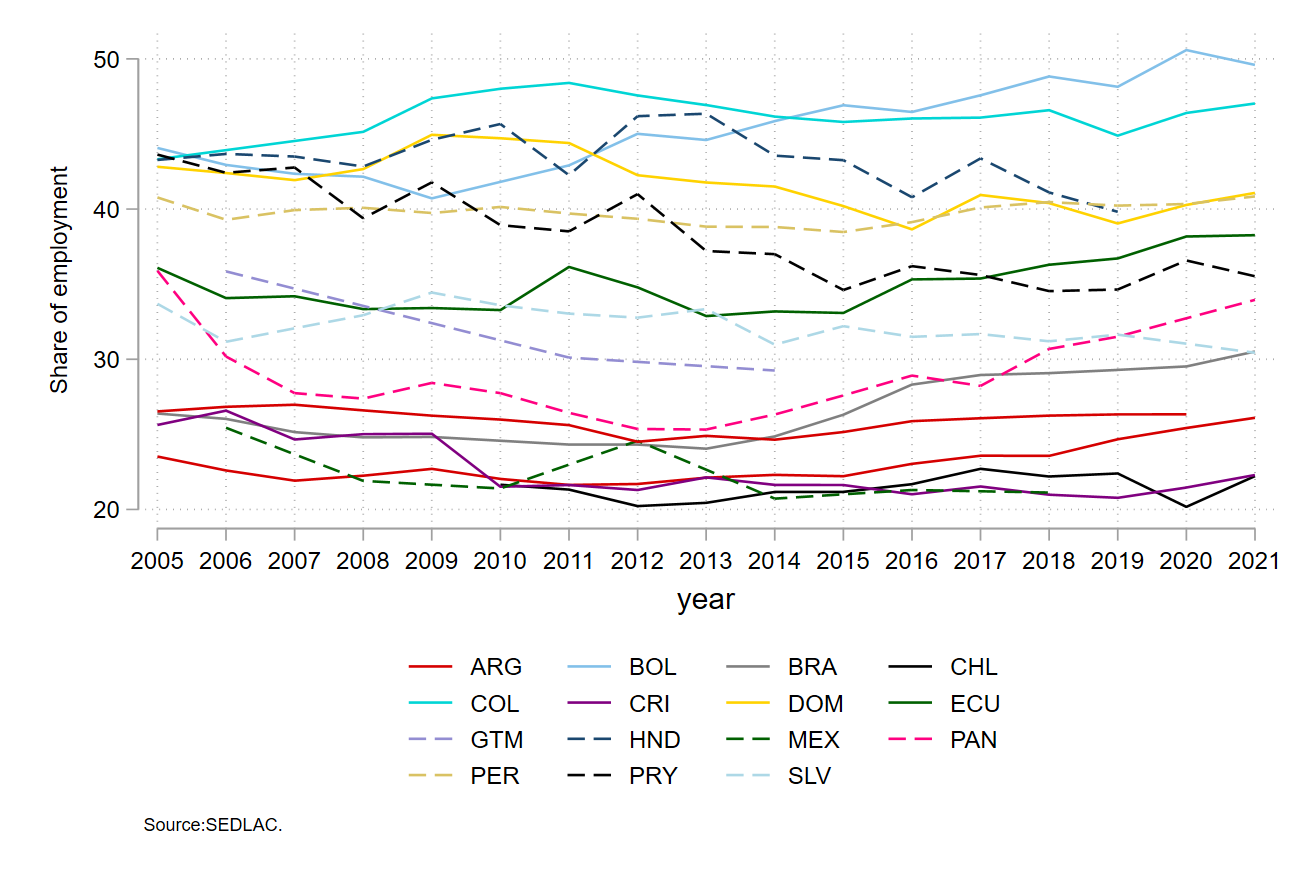
\includegraphics[width=0.8\linewidth]{latex/figures/Evolution/self_employed_all.png}
        \label{fig:Evolution_selfemployed}
        \centering
        \footnotesize{Source: Household Surveys-SEDLAC.}
 \end{figure}
 \end{frame}
%---------------------------------------------------------
%---------------------------------------------------------
\begin{frame}
\frametitle{Dynamics: last 20 years}
\begin{figure}[!htb]
        \justifying
        \caption{Self-employed workers who do not contribute to SS by country}     
        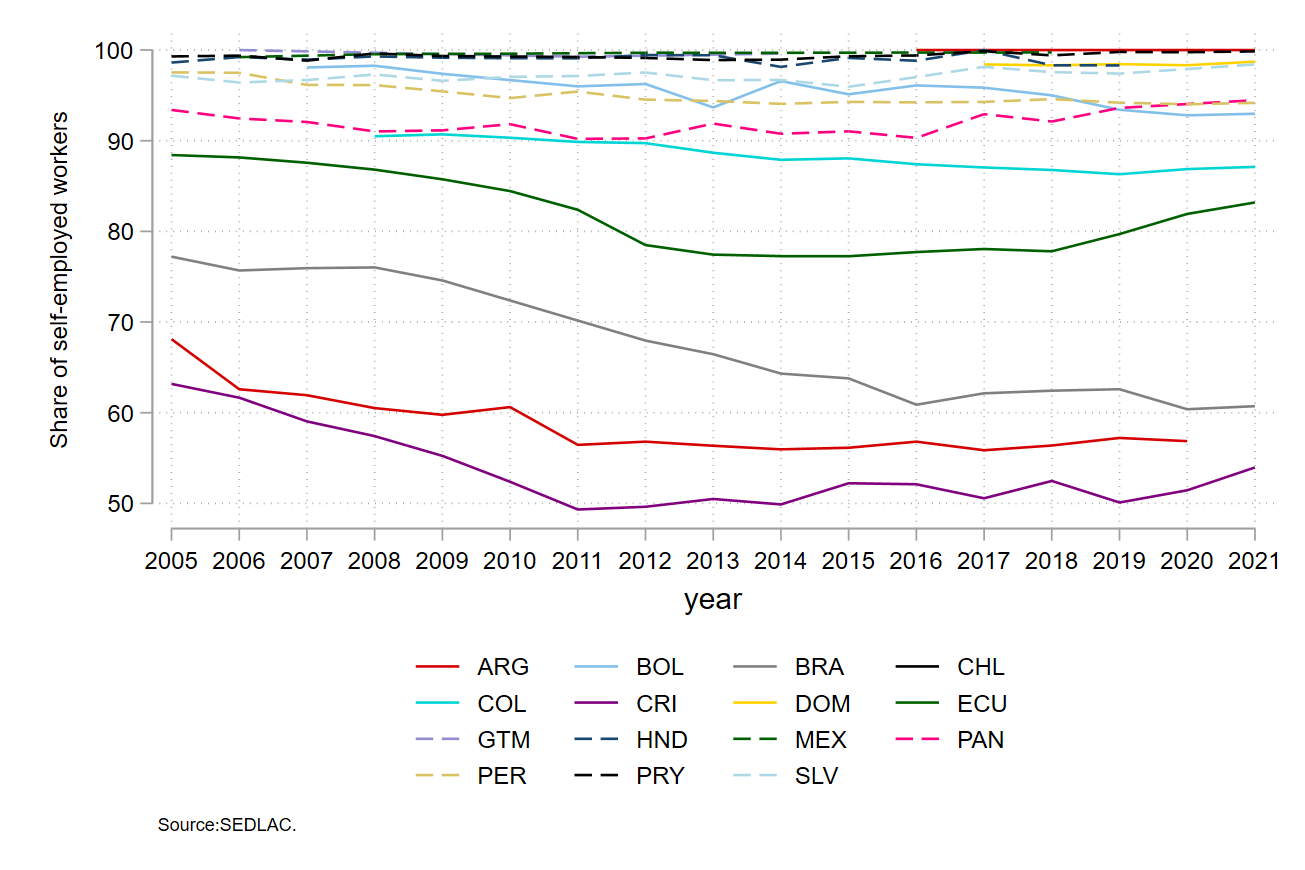
\includegraphics[width=0.8\linewidth]{latex/figures/Evolution/iss_sfemployed_all.png}
        \label{fig:Evolution_selfemployedSS}
        \centering
        \footnotesize{Source: Household Surveys-SEDLAC.}
 \end{figure}
 \end{frame}
%--------------------------------------------------------
%--------------------------------------------------------
%---------------------------------------------------------
%---------------------------------------------------------
%---------------------------------------------------------
%---------------------------------------------------------
%---------------------------------------------------------
%---------------------------------------------------------
%---------------------------------------------------------
%---------------------------------------------------------
%---------------------------------------------------------
%---------------------------------------------------------
%---------------------------------------------------------
%---------------------------------------------------------
%---------------------------------------------------------
%---------------------------------------------------------
%---------------------------------------------------------
%---------------------------------------------------------
%---------------------------------------------------------
%---------------------------------------------------------
%---------------------------------------------------------


\end{document}